\documentclass[12pt]{exam}
\usepackage[utf8]{inputenc}		% Caracteres latinos
\usepackage[spanish]{babel}		% Idioma español
\usepackage{geometry}			% Organizar el documento
\usepackage{graphicx}			% Incluir gráficos
\usepackage{makecell}			% Para personalizar las celdas de una tabla
\usepackage[nohdr]{mathexam}	% Añadimos el paquete mathexam (sin header)
\usepackage{amsmath}
\usepackage{amsfonts}
\usepackage{amssymb}
\usepackage{mathtools}
\usepackage{tikz,pgfplots}
\usepgfplotslibrary{polar}
\usepackage[shortlabels]{enumitem}
\usepackage{multirow}
 \renewcommand{\baselinestretch}{1.5}
 \setlength{\arrayrulewidth}{2mm}
\setlength{\tabcolsep}{10pt}
\renewcommand{\arraystretch}{2}
\usepackage{textpos}
\usepackage{amsmath}
\usepackage{amsfonts}
\usepackage{amssymb}
\usepackage{mathtools}
\usepackage{tikz,pgfplots}
\usepgfplotslibrary{polar}
\usepackage[shortlabels]{enumitem}
\usepackage{textpos}
\usepackage{caption}
\usepackage{mwe}
\usepackage{relsize}
 \renewcommand{\baselinestretch}{1.5}
 \usepackage{graphicx}
\newcommand\sbullet[1][.5]{\mathbin{\vcenter{\hbox{\scalebox{#1}{$\bullet$}}}}}
\usepackage{multicol}
%\usepackage[]{mathptmx}        % A free version o Times Roman with mathematical symbols
%\usepackage{pzc}               % fuente cursiva (conjuntos) Zapf Chancery
%\usepackage{showframe}
%\usepackage{lipsum}

% DOCUMENTACIÓN DE LA CLASE EXAM
% http://ftp.inf.utfsm.cl/pub/tex-archive/macros/latex/contrib/exam/examdoc.pdf
% DOCUMENTACIÓN DE LA CLASE MATHEXAM
% http://ctan.dcc.uchile.cl/macros/latex/contrib/mathexam/doc/mathexam.pdf

% Definimos la geometría de la primera página
\geometry{
	a4paper,                    % Tamaño del documento
	hmargin = {1.5cm, 1.5cm}, 	% Margen horizontal izquierdo, derecho
	vmargin = {.5cm, .2cm},	    % Margen vertical superior, inferior
	headsep = 4mm,				% Separación entre el encabezado y el texto
	head = .2cm,				% Tamaño del encabezado
	% marginparsep = 5mm, 		% Seperación entre las notas y el texto
	% marginpar = 1.5cm,		% Tamaño de las notas
	includeall,                 % incluye el encabezado, footer y notas dentro del tamaño del documento
	nomarginpar,	            % Elimina las notas
	foot = 1cm,                 % Tamaño del footer
	twoside,                	% Habilita el modo de impresión a doble cara
}

\selectlanguage{spanish}        % Selecciona el idioma
\spanishdecimal{.}

%\pagestyle{headandfoot}         % Nuestro examen tendrá encabezado y pié

% DEFINIMOS EL ENCABEZADO
%\header{
%\begin{tabular}{l c c c l}
%            \makecell{\includegraphics[height=2.5cm]{logo.png}} &
%            \makecell{\textbf{IPEA 215} \\Raúl Scalabrini Ortiz} &
%            \makecell{Examen} &
%            \makecell{Curso\\1er Año} &
%             \makecell[l]{Apellido y %Nombre:\enspace\makebox[2in]{\hrulefill}\\Fecha: \today}
%        \end{tabular}}{}{}

% DEFINIMOS EL PIE
%\rfoot{Página \thepage\ de \numpages}

% DOCUMENTO
\begin{document}


\begin{center}
\Large 
\textbf{Reposición Examen 1}
\end{center}{}
\normalsize



\pointpoints{punto}{puntos}
\pointformat{\bfseries\boldmath(\thepoints)}
\vskip10pt

\begin{questions}

\question 
¿Hay un número $a$ tal que $$\lim\limits_{x \to -2}\dfrac{3x^2+ax+a+3}{x^2+x-2}$$ exista? Si es así, encuentra los valores de $a$ y del límite. 
\vskip10pt

%\question ¿Cuál es el valor del siguiente límite: $\lim\limits_{t \to 0}\left(\dfrac{1}{t\sqrt{1+t}}-\dfrac{1}{t}\right)$?

% \question ¿Para qué valores de la constante $c$ la función $f$ es continua en $(-\infty,\infty)$?
% $$f(x) = \begin{dcases} cx+1 & \text{si } x \leq 3 \\ cx^2-1 & \text{si } x > 3 \end{dcases}$$
% \vskip10pt

   \question La siguiente figura muestra las gráficas de $f$, $f'$ y $f''$. Identifica cada curva y explica tu elección. 
   \begin{center}
  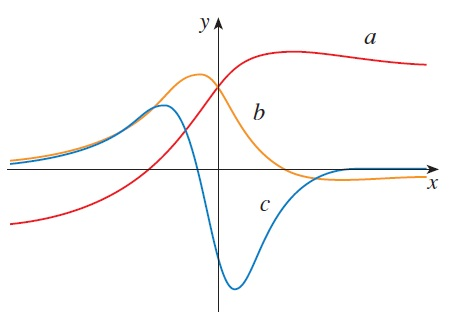
\includegraphics[scale=1]{curvas derivada.jpg}     
   \end{center}

\question El desplazamiento (en centímetros) de una partícula que se mueve en línea recta está dado por $s=10t-1.86t^2$. Encuentra la velocidad instantánea cuando $t=1$.
 \vskip10pt
\question 
Determina una ecuación de la recta tangente a la curva $y=\dfrac{x-1}{x-2}$ en el punto $(3,2)$.

\end{questions}



\newpage

\begin{center}
\Large 
\textbf{Reposición Examen 2}
\end{center}{}
\normalsize

\begin{questions}
    \question Una plataforma de perforación a 12 km de la costa debe ser conectada mediante un oleoducto a una refinería que está a 20 km en línea recta desde el punto de la costa más cercano a la plataforma. Si instalar la tubería debajo del agua cuesta \$500,000 por km y en tierra cuesta \$300,000 por km, ¿Qué combinación de instalación subacuática y terrestre da la conexión más barata?

\vskip10pt
%\question 
%Si $f(x)=ax^3+bx^2+cx+d$, determina $a$, $b$, $c$, $d$ de modo que $f$ tenga un extremo relativo en el punto $(0,3)$ y un punto de inflexión en $(1,-1)$. Dibuja la gráfica para apoyarte.
%\vskip10pt
\question Para la función $f(x)=x^4-4x^3+10$ en $[-2,4]$: i) encuentra los puntos críticos, ii) determina los extremos relativos (locales) y absolutos de la función en el intervalo, iii) determina los intervalos en los que la función es creciente o decreciente, iv) encuentra los puntos de inflexión, v) determina dónde la gráfica de la función es cóncava hacia arriba y dónde es cóncava hacia abajo. Finalmente, dibuja la gráfica de la función.

\question La ecuación $y''+y'-2y=sen\,x$ se denomina ecuación diferencial porque involucra una función desconocida y sus derivadas $y'$ y $y''$. Determina las constantes $A$ y $B$ de tal manera que la función $y=Asen\,x+Bcos\,x$ satisface esta ecuación.

    \end{questions}

\vskip30pt

\begin{center}
\Large
\textbf{Reposición Examen 2}
\end{center}{}
\normalsize

\begin{questions}
    \question Una plataforma de perforación a 12 km de la costa debe ser conectada mediante un oleoducto a una refinería que está a 20 km en línea recta desde el punto de la costa más cercano a la plataforma. Si instalar la tubería debajo del agua cuesta \$500,000 por km y en tierra cuesta \$300,000 por km, ¿Qué combinación de instalación subacuática y terrestre da la conexión más barata?

\vskip10pt
%\question 
%Si $f(x)=ax^3+bx^2+cx+d$, determina $a$, $b$, $c$, $d$ de modo que $f$ tenga un extremo relativo en el punto $(0,3)$ y un punto de inflexión en $(1,-1)$. Dibuja la gráfica para apoyarte.
%\vskip10pt
\question Para la función $f(x)=x^4-4x^3+10$ en $[-2,4]$: i) encuentra los puntos críticos, ii) determina los extremos relativos (locales) y absolutos de la función en el intervalo, iii) determina los intervalos en los que la función es creciente o decreciente, iv) encuentra los puntos de inflexión, v) determina dónde la gráfica de la función es cóncava hacia arriba y dónde es cóncava hacia abajo. Finalmente, dibuja la gráfica de la función.

\question La ecuación $y''+y'-2y=sen\,x$ se denomina ecuación diferencial porque involucra una función desconocida y sus derivadas $y'$ y $y''$. Determina las constantes $A$ y $B$ de tal manera que la función $y=Asen\,x+Bcos\,x$ satisface esta ecuación.

    \end{questions}


\newpage

\begin{center}
\Large 
\textbf{Reposición Examen 3}
\end{center}{}
\normalsize

\begin{questions}
    \question En la siguiente figura se proporciona la gráfica de una función $f$. ¿Qué gráfica es una antiderivada de $f$ y por qué?
    \begin{center}
      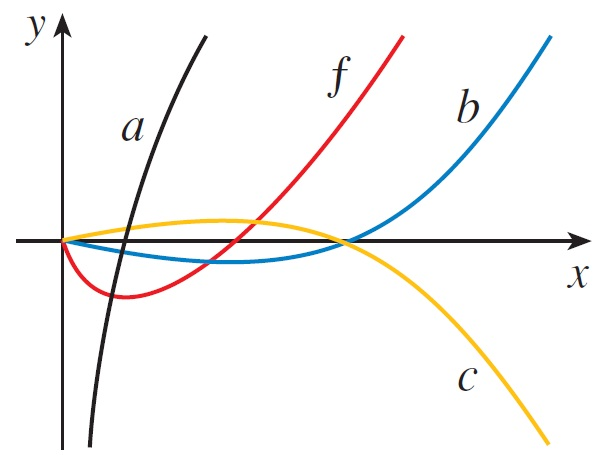
\includegraphics[scale=0.55]{curvas antiderivadas.jpg}   
    \end{center}
   
\vskip10pt

    \question Una población de abejas se inicia con 100 individuos y se incrementa en una proporción de $n'(t)$ individuos por semana. ¿Qué representa $100+\mathlarger{\int_0^{15}n'(t)\;dt}$?
    \vskip10pt
    \question Determina $f(t)$ si $f'(t)=2cos\,t+sec^2\,t$ en el intervalo $-\pi/2 < t < \pi/2$, considerando que $f(\pi/3)=4$.
\vskip12pt
\question Una partícula se mueve a lo largo de una recta con la función de velocidad $v(t)=t^2-t-6$, donde $v$ se mide en metros por segundo. Encuentra el desplazamiento y la distancia total recorrida por la partícula durante el intervalo de tiempo $[0,4]$.
    
    \end{questions}{}

\newpage
\begin{center}
\Large 
\textbf{Reposición Examen 4}
\end{center}{}
\normalsize

\begin{questions}
        \question Si la proporción de nacimientos de una población es $b(t)=4200e^{0.020t}$ personas por cada año y la de decesos es $d(t)=2180e^{0.015t}$ personas por cada año. Encuentra el área entre estas curvas para $0\leq t\leq 10$. ¿Qué representa el área?
\vskip12pt
        \question La densidad lineal de una varilla de 8 $m$ de longitud es $\rho(x)=\dfrac{12}{\sqrt{x+1}} \, kg/m$, donde $x$ se mide en metros desde un extremo de la varilla. Determina la densidad promedio de la varilla. 
\vskip12pt
 %   \question Si $f(t)$ es continua para $t\geq 0$, la \textit{transformada de Laplace de $f$} es la función de $F$ definida por $$F(s)=\displaystyle\int_0^\infty f(t)e^{-st}\;dt$$
 %   y el dominio de $F$ es el conjunto de todos los números $s$ para los que la integral converge. Encuentra la transformada de Laplace de la  función $f(t)=e^t$

    \question 
    Sea $$ f(x) = \begin{dcases} \dfrac{3}{64}\,x\sqrt{16-x^2} & \text{si } 0 \leq x \leq 4 \\ 0 & \text{si } x < 0 \quad \text{ó }\quad  x > 4 \end{dcases}$$
    \begin{enumerate}[a)]
    \item Verifica que $f$ es una función de densidad de probabilidad.
    \item Determina $P(X<2)$.
\end{enumerate}
 \vskip12pt       
\question Evalúa la siguiente integral:   
    $\mathlarger{\int ln^2x\,dx}$
    
\end{questions}{}

\vskip30pt

\begin{center}
\Large 
\textbf{Reposición Examen 4}
\end{center}{}
\normalsize

\begin{questions}
        \question Si la proporción de nacimientos de una población es $b(t)=4200e^{0.020t}$ personas por cada año y la de decesos es $d(t)=2180e^{0.015t}$ personas por cada año. Encuentra el área entre estas curvas para $0\leq t\leq 10$. ¿Qué representa el área?
\vskip12pt
        \question La densidad lineal de una varilla de 8 $m$ de longitud es $\rho(x)=\dfrac{12}{\sqrt{x+1}} \, kg/m$, donde $x$ se mide en metros desde un extremo de la varilla. Determina la densidad promedio de la varilla. 
\vskip12pt
 %   \question Si $f(t)$ es continua para $t\geq 0$, la \textit{transformada de Laplace de $f$} es la función de $F$ definida por $$F(s)=\displaystyle\int_0^\infty f(t)e^{-st}\;dt$$
 %   y el dominio de $F$ es el conjunto de todos los números $s$ para los que la integral converge. Encuentra la transformada de Laplace de la  función $f(t)=e^t$

    \question 
    Sea $$ f(x) = \begin{dcases} \dfrac{3}{64}\,x\sqrt{16-x^2} & \text{si } 0 \leq x \leq 4 \\ 0 & \text{si } x < 0 \quad \text{ó }\quad  x > 4 \end{dcases}$$
    \begin{enumerate}[a)]
    \item Verifica que $f$ es una función de densidad de probabilidad.
    \item Determina $P(X<2)$.
\end{enumerate}
 \vskip12pt       
\question Evalúa la siguiente integral:   
    $\mathlarger{\int ln^2x\,dx}$
    
\end{questions}{}


%\Large Opcional\normalsize

%Usa la técnica de \textit{Por Partes} para resolver
%$$\mathlarger{\int ln^2x\;dx}$$

%\newpage


% Geometría para la otra carilla
\newgeometry{
	hmargin = {1.5cm, 0.5cm},https://www.overleaf.com/project/5d325eec78dcb00f266b3ae0
	vmargin = {0.5cm, 1cm},
	nofoot,			% Elimina el pié
	nohead,			% Elimina el encabezado
	nomarginpar,	% Elimina las notas
	includeall,
}% \savegeometry{geometria_1}

\pagestyle{foot}    % El estilo de ésta página sólo constará de pié de página
\runningfooter{}{}{Página \thepage\ de \numpages}


%\lipsum[1-5]

% \restoregeometry
% \loadgeometry{geometria_1}


\end{document}